%%%%%%%%%%%%%%%%%%%%%%%%%%%%%%%%%%%%%%%%%
% Beamer Presentation
% LaTeX Template
% Version 1.0 (10/11/12)
%
% This template has been downloaded from:
% http://www.LaTeXTemplates.com
%
% License:
% CC BY-NC-SA 3.0 (http://creativecommons.org/licenses/by-nc-sa/3.0/)
%
%%%%%%%%%%%%%%%%%%%%%%%%%%%%%%%%%%%%%%%%%

%----------------------------------------------------------------------------------------
%	PACKAGES AND THEMES
%----------------------------------------------------------------------------------------

\documentclass{beamer}

\mode<presentation> {

% The Beamer class comes with a number of default slide themes
% which change the colors and layouts of slides. Below this is a list
% of all the themes, uncomment each in turn to see what they look like.

%\usetheme{default}
%\usetheme{AnnArbor}
%\usetheme{Antibes}
%\usetheme{Bergen}
%\usetheme{Berkeley}
%\usetheme{Berlin}
%\usetheme{Boadilla}
%\usetheme{CambridgeUS}
%\usetheme{Copenhagen}
%\usetheme{Darmstadt}
%\usetheme{Dresden}
%\usetheme{Frankfurt}
%\usetheme{Goettingen}
%\usetheme{Hannover}
%\usetheme{Ilmenau}
%\usetheme{JuanLesPins}
%\usetheme{Luebeck}
\usetheme{Madrid}
%\usetheme{Malmoe}
%\usetheme{Marburg}
%\usetheme{Montpellier}
%\usetheme{PaloAlto}
%\usetheme{Pittsburgh}
%\usetheme{Rochester}
%\usetheme{Singapore}
%\usetheme{Szeged}
%\usetheme{Warsaw}

% As well as themes, the Beamer class has a number of color themes
% for any slide theme. Uncomment each of these in turn to see how it
% changes the colors of your current slide theme.

%\usecolortheme{albatross}
%\usecolortheme{beaver}
%\usecolortheme{beetle}
%\usecolortheme{crane}
%\usecolortheme{dolphin}
%\usecolortheme{dove}
%\usecolortheme{fly}
%\usecolortheme{lily}
%\usecolortheme{orchid}
%\usecolortheme{rose}
%\usecolortheme{seagull}
%\usecolortheme{seahorse}
%\usecolortheme{whale}
%\usecolortheme{wolverine}

%\setbeamertemplate{footline} % To remove the footer line in all slides uncomment this line
%\setbeamertemplate{footline}[page number] % To replace the footer line in all slides with a simple slide count uncomment this line

%\setbeamertemplate{navigation symbols}{} % To remove the navigation symbols from the bottom of all slides uncomment this line
}

\usepackage{graphicx} % Allows including images
\usepackage{booktabs} % Allows the use of \toprule, \midrule and \bottomrule in tables
\usepackage{caption}
\usepackage{epstopdf}



%----------------------------------------------------------------------------------------
%	TITLE PAGE
%----------------------------------------------------------------------------------------

\title[Reservoir Computing]{Reservoir Computing for Neural Networks} % The short title appears at the bottom of every slide, the full title is only on the title page

\author{Felix Grezes} % Your name
\institute[CUNY] % Your institution as it will appear on the bottom of every slide, may be shorthand to save space
{
CUNY Graduate Center \\ % Your institution for the title page
\medskip
\textit{fgrezes@gc.cuny.edu} % Your email address
}
\date{September 4, 2014} 

\begin{document}

\setbeamertemplate{caption}{\raggedright\insertcaption\par}

%----------------------------------------------------------------------------------------
%	PRESENTATION SLIDES
%----------------------------------------------------------------------------------------

\begin{frame}
\titlepage % Print the title page as the first slide
\end{frame}

%----------------------------------------------------------------------------------------
\section{Introduction}

\begin{frame}
\frametitle{Introduction}

%\begin{center} 
%Central question of A.I.:
%Can human thoughts and behavior be explained and reproduced by computers?
%\end{center}

\begin{itemize}
\item The artificial neural network paradigm is a major area of research within A.I., with feedforward networks having the most recent success.
\item Recurrent networks offer more biological plausibility and theoretical computing power, but exacerbate the flaws of feedforward nets. 
\item Reservoir computing emerges as a solution, offering a generic paradigm for fast and efficient training of RNNs.
\item Used in a variety of fields: NLP, computational neuroscience, robotics, machine learning and more.
\end{itemize}

%fg:but still far away
%fg:other paradigms: logic, bayesian networks, 

\end{frame}

%----------------------------------------------------------------------------------------

\begin{frame}
\frametitle{Overview} % Table of contents slide, comment this block out to remove it
\tableofcontents % Throughout your presentation, if you choose to use \section{} and \subsection{} commands, these will automatically be printed on this slide as an overview of your presentation
\end{frame}
%----------------------------------------------------------------------------------------


\section{Neural Networks}
\subsection{Short History}

\begin{frame}
\frametitle{Short History of Neural Networks}

\begin{block}{Some Important Dates}
%fg:these are dates I consider important. barely an overview
	\begin{itemize}
	\item 1890 Discovery of the biological neuron by Golgi and Ram\'{o}n y Cajal.
    %advent of computers
    \item 1957 Rosenblatt's Perceptron:\\ $f(x) = 1$ if $w \cdot x + b>0$, and $0$ otherwise.
    \item 1969 Minsky and Papert show that perceptron cannot learn XOR 
    \item 1975 Werbos proposes the backpropagation algorithm, training over multiple layers of perceptrons.
    \item 1989/91 Cybenko/Hornik proves that multi-layer feedforward networks are universal function approximators.
	\item 1990 Werbos proposes the backpropagation through time algorithm for RNNs.
	\item 2001/02 Jaeger/Maass propose the reservoir computing paradigm, under the names of Echo State Networks/Liquid State Machines.
    \end{itemize}
   
\end{block}
\end{frame}

% fg: before continuing, 

%----------------------------------------------------------------------------------------
\subsection{Feedforward Networks}
%\subsubsection{Artificial Neuron}
\begin{frame}
\frametitle{Feedforward Networks - The Artificial Neuron}

\begin{figure}[!htbp]
\centering
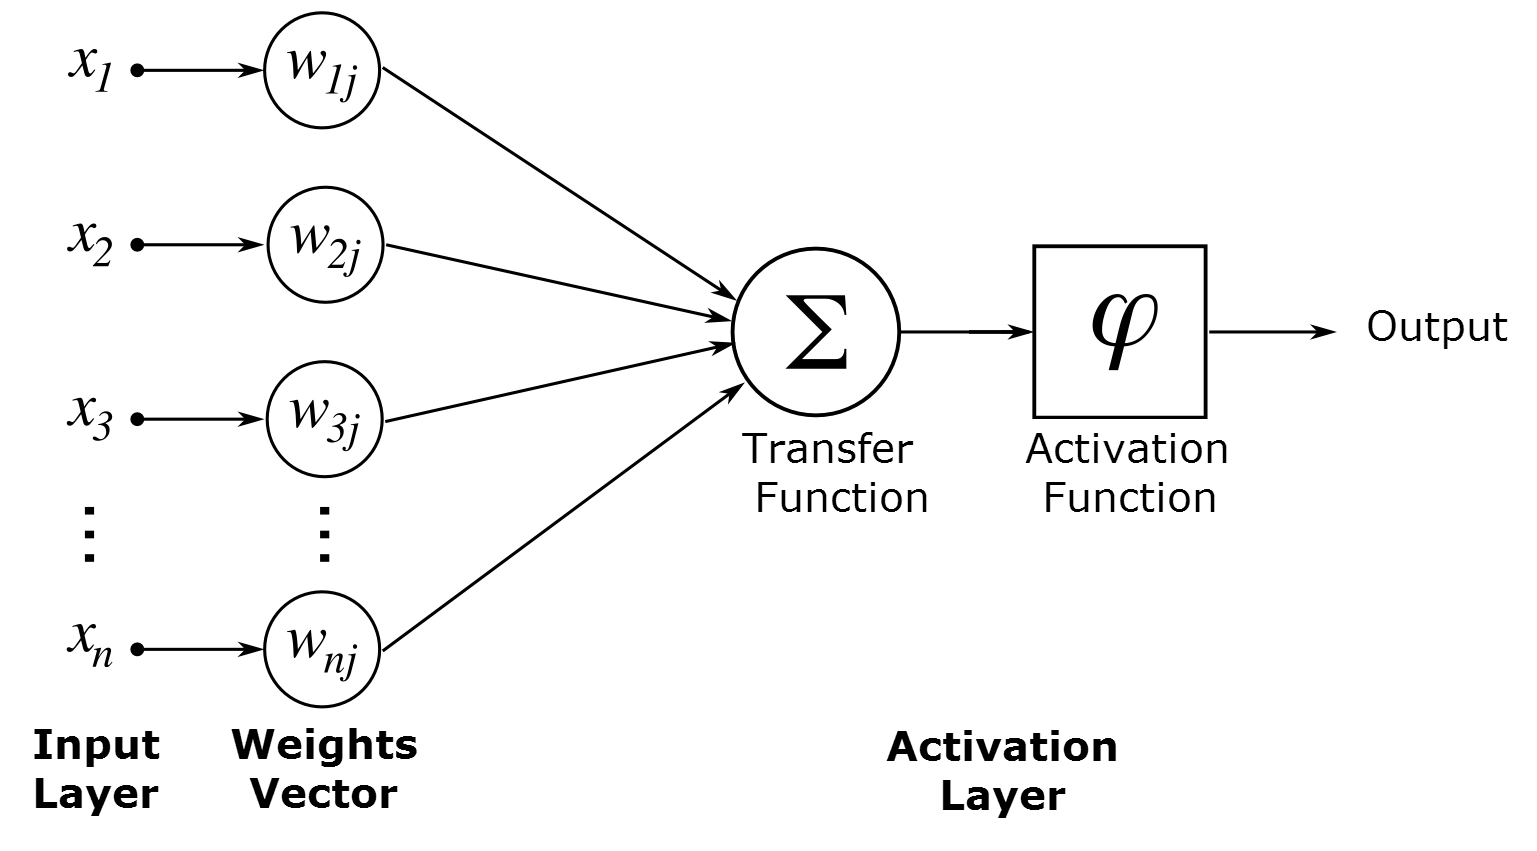
\includegraphics[width=0.9\textwidth]{pictures/ArtificialNeuronModel.png}
% \caption{Model of an Artificial Neuron}
\label{fig:neuron}
\end{figure}

% fg: non-linear activation functions: threshold (perceptron), tanh, sigmoid. esoteric: cosine

\end{frame}

%----------------------------------------------------------------------------------------
%\subsubsection{Feedforward Networks Architecture}

\begin{frame}
\frametitle{Feedforward Networks Architecture}

\begin{figure}[!htbp]
\centering
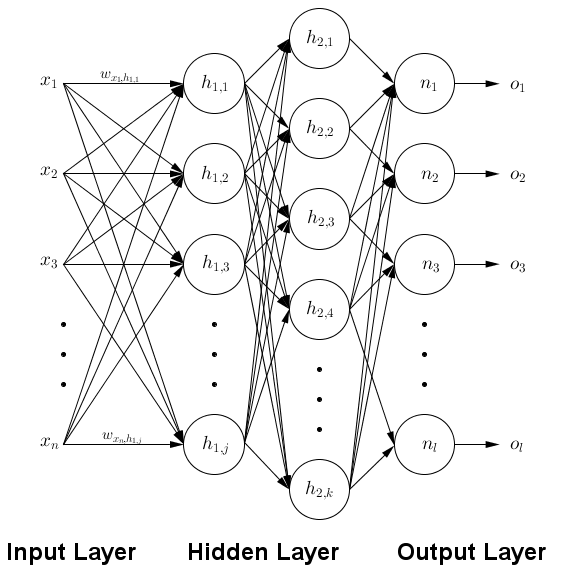
\includegraphics[width=\textwidth,height=0.85\textheight,keepaspectratio]{pictures/FeedForwardNeuralNetwork.png}
% \caption{Model of an Feedforward Neural Network}
\label{fig:feedforward}
\end{figure}

\end{frame}

%fg:does not contain cycles

%----------------------------------------------------------------------------------------
%\subsubsection{Universal Approximators}

\begin{frame}
\frametitle{Feedforward Networks - Universal Approximators}

In landmark results, Cybenko (1989) and Hornik(1991) proved that feedforward networks can approximate any continuous function from $\mathbb{R} \rightarrow \mathbb{R}$ under certain conditions:
\begin{center}
\begin{itemize}
\item The activation function needs to be continuous, non-constant, bounded, and monotonically-increasing.
%fg: all the previously mentioned functions are these
\item The network contains one or more hidden layers.
\end{itemize}
\end{center}

These results show that it is the layered architecture that gives the networks the power to approximate any function, legitimizing the search for the most efficient learning algorithms.

%fg: learning the weights

\end{frame}


%----------------------------------------------------------------------------------------
%\subsubsection{Backpropagation}

\begin{frame}
\frametitle{Backpropagation - Werbos (1975)}
The most successful training algorithm for feedforward neural networks.\\
It is a variant of gradient-descent and requires the activation function to be differentiable.

\vspace{3mm}
Steps:
\begin{enumerate}
\item Forward propagation of the input values to obtain the activation of each neuron.
\item Backwards propagation of the error for each node, in order to calculate the delta (weight update) for each weight. Computing the delta is done by using the calculus chain rule to calculate the partial derivative of the error with respect to a  weight.
\item Update each weight according to the gradient and learning rate. 
\item Repeat until the error over the data is below a threshold, or the gradient converges, or for a fixed number of iterations.
\end{enumerate}

\end{frame}
%----------------------------------------------------------------------------------------

%give some criticism of Backprop
%allude to the vanishing gradient problem that we will return too
%talk a bit about recent success of FFNNs

%----------------------------------------------------------------------------------------
\subsection{Recurrent Neural Networks}

\begin{frame}
\frametitle{Recurrent Neural Networks}
\begin{center}
Recurrent Neural Networks contain cycles in the graph.
\begin{figure}[!htbp]
\centering
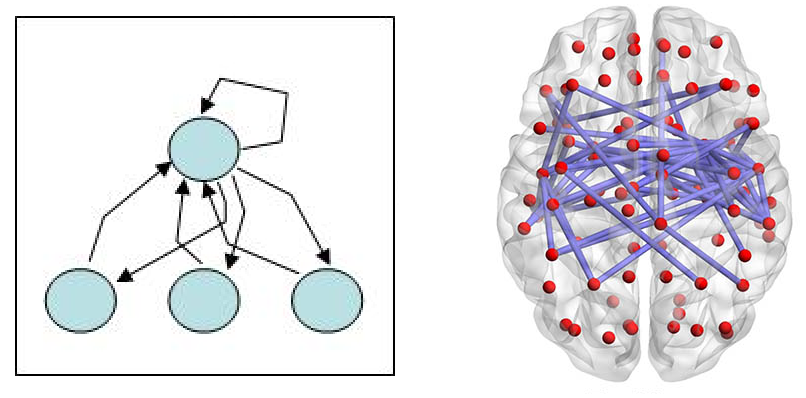
\includegraphics[width=0.6\textwidth]{pictures/rnn_brain.png}
%\caption{Model of a a small Recurrent Neural Network. Image from \cite{rnn} }
\label{fig:rnn}
\end{figure}
\end{center}

\begin{block}{Why study recurrent neural networks?}

\begin{itemize}
\item The human brain has a recurrent architecture. Computational neuroscientists need to understand how RNNs work.
\item Because of the recurrent architecture, RNNs approximate not just functions but dynamical systems.
\end{itemize}

\end{block}

\end{frame}

%----------------------------------------------------------------------------------------
%\subsubsection{Dynamical Systems}

\begin{frame}
\frametitle{RNNs - Dynamical Systems}
\begin{block}{Definition}
A discrete dynamical system is defined by a state $x \in X$ (state space) that evolves over discrete time-steps according to a fixed rule $f$.\\
The rule $f$ is a function of time and the initial state $x_0$, and $f(x_0, t)$ it the state at time-step $t$.
\end{block}
%Turing machines are dynamical systems
\vspace{0.8mm}

Dynamical system are famous for their long term dependencies and sensitivity to small initial changes (Chaos Theory).
%chaos theory
\vspace{0.9mm}

RNNs can model complex dynamical systems, allowing them to  'remember' input values over time by echoing them through the network nodes. This is particularly useful for tasks with temporal dependencies.
\vspace{0.9mm}

Feedforward networks have relied on hand-crafted data representation, e.g. n-grams in NLP tasks.

\end{frame}

%----------------------------------------------------------------------------------------
%\subsubsection{Training RNNs}

\begin{frame}
\frametitle{Training RNNs}
\begin{block}{Universal Approximator Theorem - Siegelmann and Sontag (1991)}
Similar to feedforward networks, RNNs are universal approximators of dynamical systems, proved by emulating a universal Turing machine.
\end{block}

\begin{block}{Backpropagation Through Time - Werbos (1990)}
 Adapts the backpropagation algorithm by 'unfolding' the RNN into a feedforward network at each time step. The related weights are tied by averaging the changes after each iteration.
\begin{figure}[!htbp]
\centering
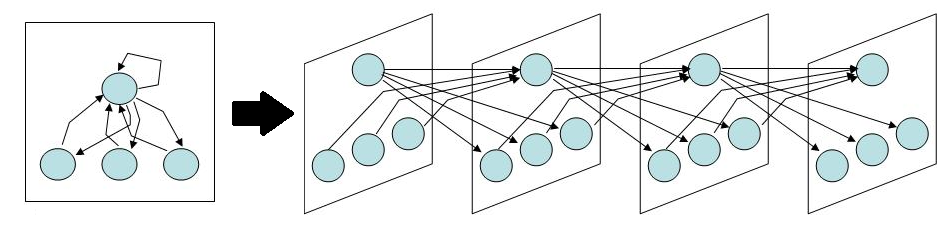
\includegraphics[width=0.9\textwidth]{pictures/bptt.png}
%\caption{Visualization of Backpropagation Through Time unfolding the RNN.}
\label{fig:bptt}
\end{figure}
\end{block}
\end{frame}

%----------------------------------------------------------------------------------------
%\subsubsection{The Vanishing Gradient Problem}
%move to RNN-BPTT section?

\begin{frame}
\frametitle{The Vanishing Gradient Problem - Hochreiter (1991)}

\begin{itemize}
\item In networks with many hidden layers, the error gradient weakens as it moves from the back of the network to the front.
\item RNNs trained with BPTT exacerbate the problem since the number of layers grows over time.
\item Schiller and Steil (2005) verified this effect experimentally, noticing that dominant changes during training only appeared on the output layer of the network.
\end{itemize}

\begin{center}
The reservoir computing paradigm emerges as a solution.
%among others: long-short term memory being the most popular
\end{center}

\end{frame}


%----------------------------------------------------------------------------------------
\section{The Reservoir Computing Paradigm}

\begin{frame}
\frametitle{The Reservoir Computing Paradigm for RNNs}
\begin{block}{Central Idea}
Since only the changes in the output layer weights are significant, then the treatment of the weights of the inner network can be {\itshape completely separated} from the treatment the output layer weights.
\end{block}

In many practical applications, the initial weights of the network are randomized and never changed, with only the weights of the output layer being trained, usually by a simple linear classifier such as logistic regression or the least squares.

\begin{figure}[!htbp]
\centering
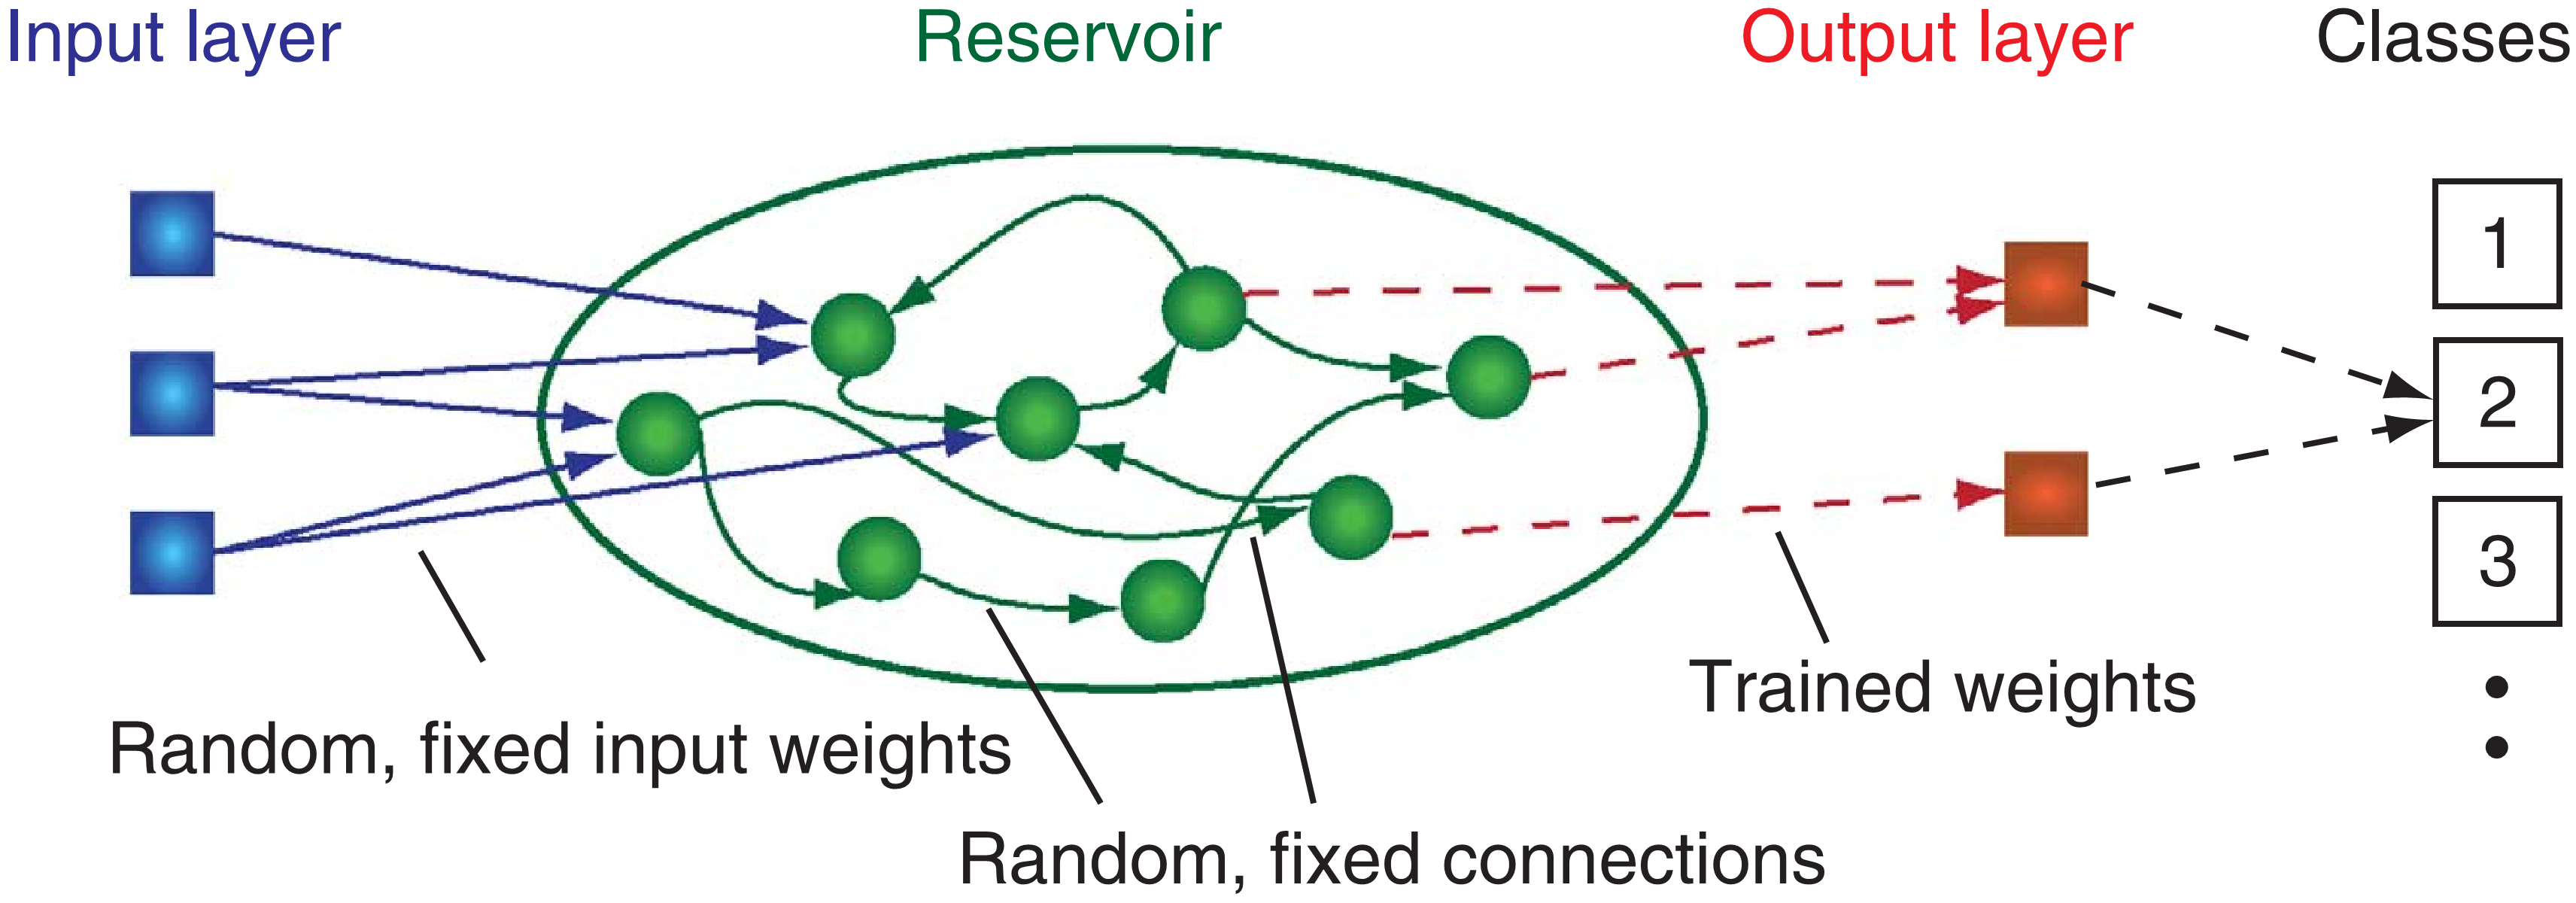
\includegraphics[width=0.7\textwidth]{pictures/reservoir_network.png}
%\caption{Model of a Reservoir Neural Network. Image from \textit{Information Processing using a Single Dynamical Node as Complex System} by Appeltant et al. \cite{appeltant2011information} }
\label{fig:reservoir}
\end{figure}

\end{frame}


%----------------------------------------------------------------------------------------
\subsection{Models}

\begin{frame}
\frametitle{Reservoir Models}
The idea of reservoir computing was proposed independently by multiple teams in the early 2000s. Since 2008, they have been united under the reservoir term.

\begin{block}{Echo State Networks - Jaeger (2001)}
Pioneered by Jaeger and his team. Their work focused on the properties of reservoir networks that make them work, and applied them to signal processing tasks, from a machine learning angle.
%sigmoid, random networks
\end{block}

\begin{block}{Liquid State Machines - Maass (2002)}
Proposed by Maass, LSMs are the other pioneer model of reservoir computing. Coming from a neuroscience background, this type of reservoir has been used to understand the computing power of real neural circuits.
%contrasts by using integraet and fire neurons, and bio-inspired 
\end{block}
\end{frame}

%----------------------------------------------------------------------------------------

\begin{frame}
\frametitle{Other Models}
The reservoir computing paradigm can be extended beyond neural networks.
\begin{block}{Water Basin - Fernando (2003)}
Taking the idea of a reservoir and echoes literally, an experiment was set up where the inputs were projected into a bucket of water, and by recording the waves bouncing around the liquid's surface, the authors were able to successfully train a pattern recognizer.
\end{block}

\begin{block}{Bacteria Colony - Fernando(2007)}
 Another exotic idea for an untrained reservoir is an E.Coli. bacteria colony, with chemical stimuli as input and protein measures as output.
\end{block}

\end{frame}
%----------------------------------------------------------------------------------------

\begin{frame}
\frametitle{Why do untrained reservoirs work?}

All these reservoir models rely on exploding the data dimensions in a random or untrained manner, where it can then be easily classified.

\begin{figure}[!htbp]
\centering
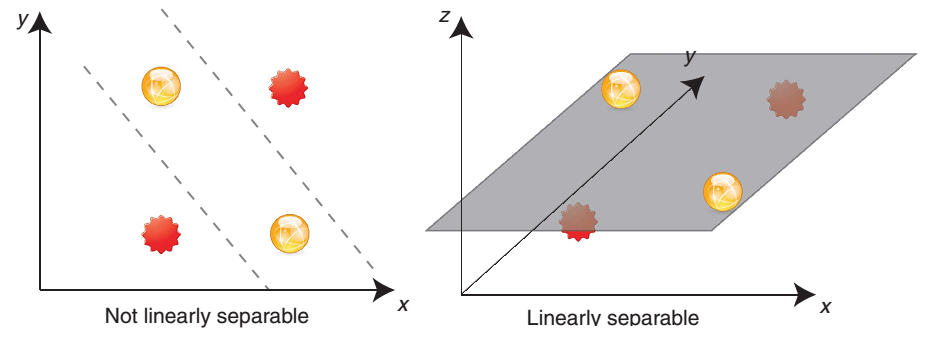
\includegraphics[width=0.9\textwidth]{pictures/dim-explo.png}
\label{fig:dim-explo}
\end{figure}

\end{frame}


%----------------------------------------------------------------------------------------
\subsection{Reservoir Computing Theory}
%fg: the following are good practices to build useful reservoirs
%\subsubsection{Echo State Property}

\begin{frame}
\frametitle{Reservoir Computing Theory - Echo State Property}
Because of the network cycles, node activities can be self-reinforcing, leading to a saturation of the network. To avoid this, reservoir networks should possess the Echo State Property.
\begin{block}{Definition: Echo State Property}
The influence of past inputs and past states over the network activities should gradually vanish over time.
\end{block}
\begin{block}{Heuristics}
\begin{itemize}
\item Scale the weights of the network to a desired spectral radius of the weight matrix.
\item A spectral radius smaller than 1 guarantees the echo state property.
\item For practical tasks with long range time dependencies, the spectral radius should be close to 1 or slightly larger.
%fg: the spectral radius is a crude measure of non-linearity in the network.
\end{itemize}
\end{block}

\end{frame}

%----------------------------------------------------------------------------------------
%\subsubsection{Separability}

\begin{frame}
\frametitle{Reservoir Computing Theory - Separability}
If two different input signals produce a similar output signal, then the output layer classifier will fail.\\
To produce reservoirs with a high separability power, the network should be:
\begin{itemize}
\item Large, allowing numerous activations.
\item Sparse, making the activations decoupled.
\end{itemize}
\vspace{0.8mm}
When producing random reservoirs, their separability power can be compared by measuring the distances between states of different inputs.
%fg: give two reservoir the same inputs, see which one makes states the further apart.
\end{frame}

%----------------------------------------------------------------------------------------
%\subsubsection{Topology}

\begin{frame}
\frametitle{Reservoir Computing Theory - Topology}
The best topology for a reservoir network remains an open question, and certainly task dependent.
\vspace{0.8mm}

A study by Liebald (2004) compared well known topologies on dynamical system prediction tasks, including small world, scale free, biologically inspired, and exhaustively searching very small networks.
\vspace{0.8mm}

No specific topology performed better than fully random networks.
\begin{figure}[!htbp]
\centering
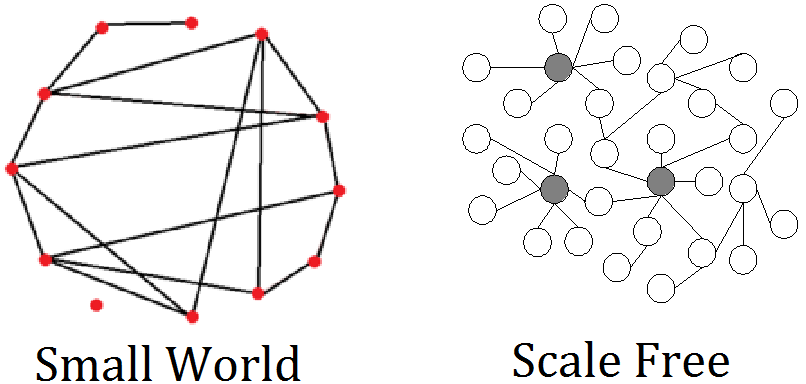
\includegraphics[width=0.6\textwidth]{pictures/top-ex.png}
%\caption{Model of a Reservoir Neural Network. Image from \textit{Information Processing using a Single Dynamical Node as Complex System} by Appeltant et al. \cite{appeltant2011information} }
\label{fig:top-ex}
\end{figure}

\end{frame}


%----------------------------------------------------------------------------------------
\section{How the Reservoir Computing Paradigm is used}

\begin{frame}
\frametitle{How the Reservoir Computing Paradigm is used}

Since the discovery of reservoir computing in the early 2000s, it has been applied in a number of tasks.
\begin{itemize}
\item Computational Neuroscience
\item Machine Learning
\item Speech Processing
\item Physics: Hardware Implementation
\end{itemize}

\end{frame}

%----------------------------------------------------------------------------------------

\begin{frame}
\frametitle{Research using Reservoirs}

The use of reservoir in scientific research can be broadly classified in two categories:
\begin{itemize}
\item Used as a generic and powerful machine learning tool.
\item Used to explain and simulate realistic biological processes.
\end{itemize}

\end{frame}


%----------------------------------------------------------------------------------------
%\subsection{Neuroscience}

\begin{frame}
\frametitle{Reservoirs in Neuroscience - Dominey (1995)}
\begin{itemize}
\item Dominey was the first to exhibit reservoir patterns in the brain, as early as 1995, before the reservoir computing was coined.
\item He was the first to spell out that some parts of the brain seemed to be randomly connected and did not change over time, and that learning only happened on the output layer. 
\item In this early work, the activity of the pre-frontal cortex was simulated using leaky-integrator neurons and the least-mean squares output classifier.
\end{itemize}
\end{frame}


%----------------------------------------------------------------------------------------
\begin{frame}
\frametitle{Reservoirs in Neuroscience - Bernacchia (2011)}

The authors found that monkey brains exhibit multiple timescales when processing expected rewards. Classical reinforcement learning only accounts for a fixed timescale.
\begin{block}{What was observed}
The activation of different blocks of neuron correlated with when the monkey expected a reward.
\end{block} 

\begin{block}{How this was reproduced}
Single 1000 neuron reservoir, with sparse and random connections. The simulations showed a similar distribution of timescales in neural activation.
\end{block}

\end{frame}

%----------------------------------------------------------------------------------------
\begin{frame}
\frametitle{Reservoirs in Neuroscience - Hinaut (2014)}
Combines research from neuroscience, robotics and linguistics to show that an iCub robot can learn complex grammar systems through purely associative mechanisms observed in its environment.
\begin{figure}[!htbp]
\centering
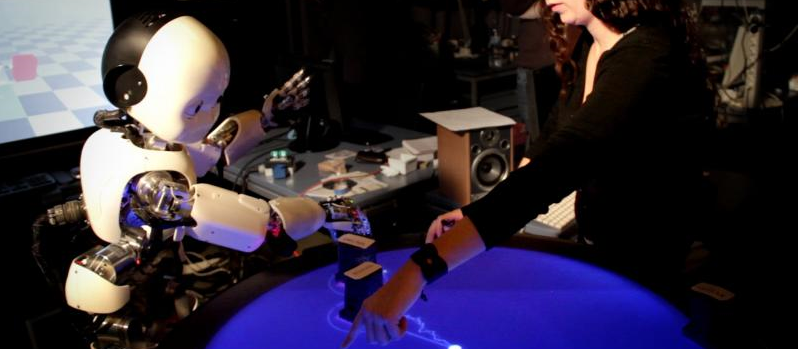
\includegraphics[width=0.6\textwidth]{pictures/icub.png}
\caption{The iCub robot learning from its environment}
\label{fig:icub}
\end{figure}
\vspace{-7mm}
By using a reservoir network modeled after the human pre-frontal cortex, the robot learns that sentences like "John hit Mary" and "Mary was hit by John" have the same meaning and same grammatical structure.


\end{frame}

%----------------------------------------------------------------------------------------
\begin{frame}
\frametitle{What do Reservoirs bring to Neuroscience?}
\begin{center}
Some kind of learning must be going on in the recurrent networks that are animal brains. But from a purely mechanical viewpoint, is it realistic that errors can influence every single connection between neurons?
\end{center}

If efficient training of RNNs is possible using the reservoir computing paradigm, it may drastically simplify the chemical mechanisms needed to explain the learning capacities of the brain.\\
Neuroscientists could confirm or refute this hypothesis with precise observations of neural activities.

\end{frame}

%----------------------------------------------------------------------------------------
%\subsubsection{Machine Learning}

\begin{frame}
\frametitle{Reservoirs in Machine Learning - Oubbati (2012)}

\begin{block}{Multi-objective Problems}
Multi-objective tasks seeks a solution that balances multiple goals at the same time: speed/quality, financial/social.
\end{block}
\vspace{5mm}

The authors used a technique called Adaptive Dynamic Programming developed to solve these multi-objective tasks, but needed a fast and powerful "critic" to compute multiple expected rewards at once.\\
\vspace{5mm}
Reservoir networks satisfy these criteria and proved capable of reaching different Pareto optimal solutions, depending on the preferences of the critic.
%ADP isi beyond the scope of this survey

\end{frame}

%----------------------------------------------------------------------------------------
%\subsubsection{Speech Processing}

\begin{frame}
\frametitle{Reservoirs in Speech Processing - Triefenbach (2010)}

Can reservoir networks compete with other state of the art techniques (HMM, Deepf Belief Nets) on the task of continuous phoneme recognition on the TIMIT dataset?
\begin{figure}[!htbp]
\centering
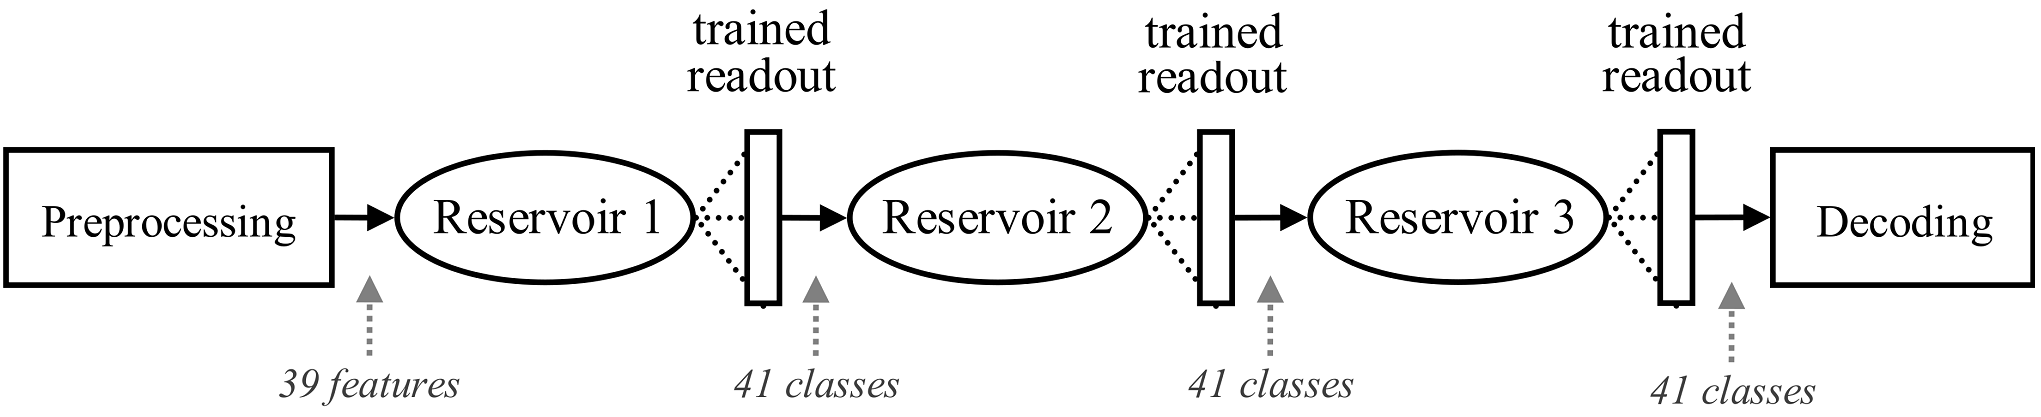
\includegraphics[width=0.9\textwidth]{pictures/layered-res.png}
\end{figure}
%describe orally the process: MFCCS etc...


\begin{block}{Results}
The overall performance was  comparable to more sophisticated approaches.\\
The second layers improves the recognition rate by 3-5\%, but subsequent layers only provide minimal gain. 
\end{block}
\end{frame}

%----------------------------------------------------------------------------------------
\begin{frame}
\frametitle{What do Reservoirs bring to Machine Learning?}

The reservoir computing paradigm provides scientists with a generic and powerful tool to tackle tasks that require temporal dependencies, without requiring hand-crafted data representations.\\
\vspace{5mm}
With the above early successes, the path is clear for other fields to use the paradigm. Simple ideas: continuous hand-written character recognition, stock market predictions, live translation...

\end{frame}


%----------------------------------------------------------------------------------------
%\subsubsection{Hardware Implementation}

\begin{frame}
\frametitle{Hardware Implementation - Appeltant 2011}

Hardware implementation are always much faster than computer simulation. However, it is both expensive to create random circuitry, and inefficient since not all random topologies possess the appropriate properties.\\
\vspace{3mm}
The authors test a tunable dynamical system, whose values are saved for a number of time-step. These delayed values act as virtual nodes of the reservoir, whose connections to the output layer a trained in classical reservoir fashion.

\begin{block}{The Mackey-Glass oscillator}
 The state $X$ evolves according to $\dot X (t) = -X(t) + \frac{\eta \cdot [X(t-\tau) + \gamma \cdot J(t)]}{[1+X(t-\tau) + \gamma \cdot J(t)]^p }$\\
with $\eta, \gamma, p$ tunable parameters. $J(t)$ is the input vector.
%explainthe oscillator, give tasks and  results
\end{block}
\end{frame}

%----------------------------------------------------------------------------------------
\subsection{Other Randomized Networks}

\begin{frame}
\frametitle{Other Randomized Networks}
The idea of separating the treatment of the output layer from the inner layers has also been applied to feedforward networks.

\begin{block}{Extreme Learning Machines - Huang (2011)}
\begin{itemize}
\item Randomize weights for the hidden layers.
\item Train only weights of the output layer.
\end{itemize}
\end{block}
ELMs have also been proven to be universal approximators, and applied to both toy tasks and real world problems.

\end{frame}


%----------------------------------------------------------------------------------------
\section{Conclusion}

\begin{frame}
\frametitle{Conclusion}
\begin{itemize}
\item The simple reservoir computing paradigm states that recurrent neural networks can be efficiently trained by optimizing only the weights connected to the output neurons, leaving the weights of internal connections unchanged. 
\item The reservoir computing paradigm offers a theoretically sound approach to modeling dynamical systems with temporal dependencies. 
\item The paradigm also promises to be much more computationally efficient than traditional RNN approaches that aim at optimizing every weight of the network.
\item Reservoir computing techniques have successfully been applied to classical artificial intelligence problems, providing state-of-the-art performance on engineering problems, and offering explanations of biological brain processes.
\end{itemize}

\end{frame}

%----------------------------------------------------------------------------------------
\subsection{Future Work using Reservoirs}

\begin{frame}
\frametitle{Future Work using Reservoirs}
\begin{itemize}
\item Speech Lab $@$ Queens College: speech prosody analysis.
\item NSF IGERT: Multi-disciplinary work (bio-medical data)
\end{itemize}

 I have already explored toy problems using reservoir networks, implemented using the OGER Python toolbox.
\begin{figure}[!htbp]
\centering
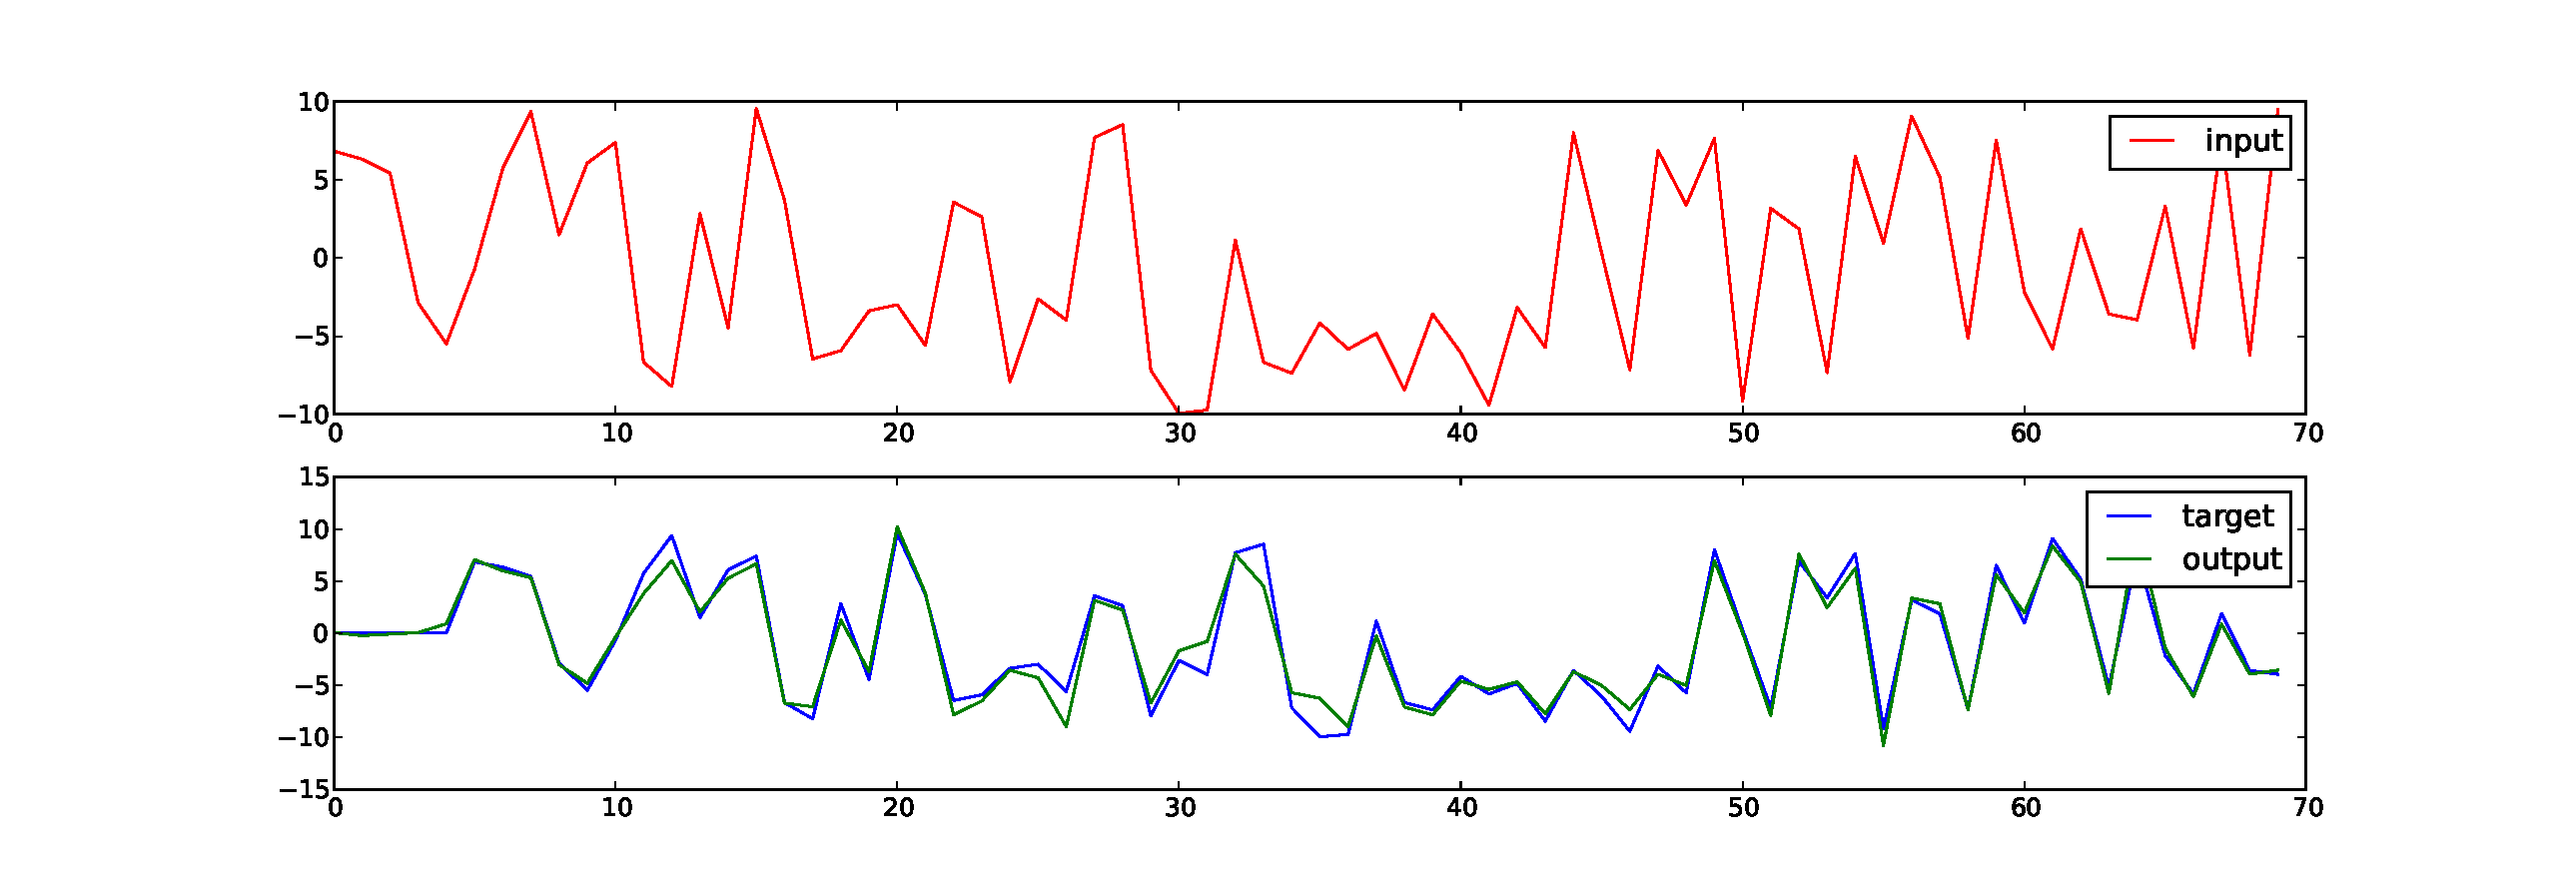
\includegraphics[width=0.8\textwidth]{pictures/my-res1.eps}
\caption{Results of a simple 50 neuron random reservoir on a k-delay replication task}
\label{fig:myres}
\end{figure}

\end{frame}
%
%%----------------------------------------------------------------------------------------
%\subsubsection{}
%
%\begin{frame}
%\frametitle{}
%
%\end{frame}



%------------------------------------------------

%\begin{frame}
%\frametitle{References}
%\footnotesize{
%\begin{thebibliography}{99} % Beamer does not support BibTeX so references must be inserted manually as below
%\
%\end{thebibliography}
%}
%\end{frame}


% %------------------------------------------------
% \section{First Section} % Sections can be created in order to organize your presentation into discrete blocks, all sections and subsections are automatically printed in the table of contents as an overview of the talk
% %------------------------------------------------

% \subsection{Subsection Example} % A subsection can be created just before a set of slides with a common theme to further break down your presentation into chunks

% \begin{frame}
% \frametitle{Paragraphs of Text}
% Sed iaculis dapibus gravida. Morbi sed tortor erat, nec interdum arcu. Sed id lorem lectus. Quisque viverra augue id sem ornare non aliquam nibh tristique. Aenean in ligula nisl. Nulla sed tellus ipsum. Donec vestibulum ligula non lorem vulputate fermentum accumsan neque mollis.\\~\\

% Sed diam enim, sagittis nec condimentum sit amet, ullamcorper sit amet libero. Aliquam vel dui orci, a porta odio. Nullam id suscipit ipsum. Aenean lobortis commodo sem, ut commodo leo gravida vitae. Pellentesque vehicula ante iaculis arcu pretium rutrum eget sit amet purus. Integer ornare nulla quis neque ultrices lobortis. Vestibulum ultrices tincidunt libero, quis commodo erat ullamcorper id.
% \end{frame}

% %------------------------------------------------
%
%\begin{frame}
%\frametitle{Bullet Points}
%\begin{itemize}
%\item Lorem ipsum dolor sit amet, consectetur adipiscing elit
%\item Aliquam blandit fauxcibus nisi, sit amet dapibus enim tempus eu
%\item Nulla commodo, erat quis gravida posuere, elit lacus lobortis est, quis porttitor odio mauris at libero
%\item Nam cursus est eget velit posuere pellentesque
%\item Vestibulum faucibus velit a augue condimentum quis convallis nulla gravida
%\end{itemize}
%\end{frame}
%
%% %------------------------------------------------
%
%\begin{frame}
%\frametitle{Blocks of Highlighted Text}
%\begin{block}{Block 1}
%Lorem ipsum dolor sit amet, consectetur adipiscing elit. Integer lectus nisl, ultricies in feugiat rutrum, porttitor sit amet augue. Aliquam ut tortor mauris. Sed volutpat ante purus, quis accumsan dolor.
%\end{block}
%
%\begin{block}{Block 2}
%Pellentesque sed tellus purus. Class aptent taciti sociosqu ad litora torquent per conubia nostra, per inceptos himenaeos. Vestibulum quis magna at risus dictum tempor eu vitae velit.
%\end{block}
%
%\begin{block}{Block 3}
%Suspendisse tincidunt sagittis gravida. Curabitur condimentum, enim sed venenatis rutrum, ipsum neque consectetur orci, sed blandit justo nisi ac lacus.
%\end{block}
%\end{frame}
%
%%------------------------------------------------
%
%\begin{frame}
%\frametitle{Multiple Columns}
%\begin{columns}[c] % The "c" option specifies centered vertical alignment while the "t" option is used for top vertical alignment
%
%\column{.45\textwidth} % Left column and width
%\textbf{Heading}
%\begin{enumerate}
%\item Statement
%\item Explanation
%\item Example
%\end{enumerate}
%
%\column{.5\textwidth} % Right column and width
%Lorem ipsum dolor sit amet, consectetur adipiscing elit. Integer lectus nisl, ultricies in feugiat rutrum, porttitor sit amet augue. Aliquam ut tortor mauris. Sed volutpat ante purus, quis accumsan dolor.
%
%\end{columns}
%\end{frame}
%
%%------------------------------------------------
%%\section{Second Section}
%%------------------------------------------------
%
%\begin{frame}
%\frametitle{Table}
%\begin{table}
%\begin{tabular}{l l l}
%\toprule
%\textbf{Treatments} & \textbf{Response 1} & \textbf{Response 2}\\
%\midrule
%Treatment 1 & 0.0003262 & 0.562 \\
%Treatment 2 & 0.0015681 & 0.910 \\
%Treatment 3 & 0.0009271 & 0.296 \\
%\bottomrule
%\end{tabular}
%\caption{Table caption}
%\end{table}
%\end{frame}
%
%%------------------------------------------------
%
%\begin{frame}
%\frametitle{Theorem}
%\begin{theorem}[Mass--energy equivalence]
%$E = mc^2$
%\end{theorem}
%\end{frame}
%
%%------------------------------------------------
%
%\begin{frame}[fragile] % Need to use the fragile option when verbatim is used in the slide
%\frametitle{Verbatim}
%\begin{example}[Theorem Slide Code]
%\begin{verbatim}
%\begin{frame}
%\frametitle{Theorem}
%\begin{theorem}[Mass--energy equivalence]
%$E = mc^2$
%\end{theorem}
%\end{frame}\end{verbatim}
%\end{example}
%\end{frame}
%
%%------------------------------------------------
%
%\begin{frame}
%\frametitle{Figure}
%Uncomment the code on this slide to include your own image from the same directory as the template .TeX file.
%%\begin{figure}
%%\includegraphics[width=0.8\linewidth]{test}
%%\end{figure}
%\end{frame}
%
%%------------------------------------------------
%
%\begin{frame}[fragile] % Need to use the fragile option when verbatim is used in the slide
%\frametitle{Citation}
%An example of the \verb|\cite| command to cite within the presentation:\\~
%
%This statement requires citation \cite{p1}.
%\end{frame}
%
%%------------------------------------------------
%
%\begin{frame}
%\frametitle{References}
%\footnotesize{
%\begin{thebibliography}{99} % Beamer does not support BibTeX so references must be inserted manually as below
%\bibitem[Smith, 2012]{p1} John Smith (2012)
%\newblock Title of the publication
%\newblock \emph{Journal Name} 12(3), 45 -- 678.
%\end{thebibliography}
%}
%\end{frame}
%
%%------------------------------------------------
%
\begin{frame}
\frametitle{\centerline{The End}}
\Huge{\centerline{Thank You}}
\end{frame}

%----------------------------------------------------------------------------------------

\end{document}